% The document class supplies options to control rendering of some standard
% features in the result.  The goal is for uniform style, so some attention 
% to detail is *vital* with all fields.  Each field (i.e., text inside the
% curly braces below, so the MEng text inside {MEng} for instance) should 
% take into account the following:
%
% - author name       should be formatted as "FirstName LastName"
%   (not "Initial LastName" for example),
% - supervisor name   should be formatted as "Title FirstName LastName"
%   (where Title is "Dr." or "Prof." for example),
% - degree programme  should be "BSc", "MEng", "MSci", "MSc" or "PhD",
% - dissertation title should be correctly capitalised (plus you can have
%   an optional sub-title if appropriate, or leave this field blank),
% - dissertation type should be formatted as one of the following:
%   * for the MEng degree programme either "enterprise" or "research" to
%     reflect the stream,
%   * for the MSc  degree programme "$X/Y/Z$" for a project deemed to be
%     X%, Y% and Z% of type I, II and III.
% - year              should be formatted as a 4-digit year of submission
%   (so 2014 rather than the accademic year, say 2013/14 say).
%
% Note there is a *strict* requirement for the poster to be in portrait 
% format so that we display them on the poster boards available.

\documentclass[ % the name of the author
                    author={Dominic Hutchinson},
                % the name of the supervisor
                supervisor={Dr. Christian Konrad},
                % the degree programme
                    degree={MEng Maths  and Computer Science},
                % the dissertation    title (which cannot be blank)
                     title={Implementing and Evaluating Space Efficient Algorithms for Detecting Large Neighbourhoods in Graph Streams},
                % the dissertation subtitle (which can    be blank)
                  subtitle={},
                % the dissertation     type
                      type={Research},
                % the year of submission
                      year={2020} ]{poster}

\usepackage[ruled, vlined]{algorithm2e}
\SetAlFnt{\small}
\SetAlCapFnt{\small}
\SetAlCapNameFnt{\small}
\usepackage{algcompatible}
\usepackage{graphicx}

\begin{document}

% -----------------------------------------------------------------------------

\begin{frame}{} 

\vfill

\begin{columns}[t]
  \begin{column}{0.900\linewidth}
  \begin{block}{\Large Graph Streams \& The $\mathtt{Neighbourhood\ Detection\ Problem}$}
 	\noindent
	Graph Streams are a sequence of instructions which describe how to construct a graph. Each instruction provides details about an edge in the graph. Graph Streams come in two forms
	\begin{itemize}
		\item \textit{Insertion-Only Streams} only ever insert new edges into the graph with each instruction.
		\item \textit{Insertion-Deletion Streams} either insert a new edge, or remove an existing edge, from the graph with each instruction.
	\end{itemize}
	In the $\mathtt{Neighbourhood\ Detection\ Problem}(n,d)$ we are given a graph with $n$ vertices \& at least one vertex of degree $d$. We are tasked to return a vertex with at least $\frac{d}c$ of its neighbours, from some approximation factor $c\geq1$.\\
	\noindent
	There are some good motivativing applications of the $\mathtt{Neighbourhood\ Detection\ Problem}$.
	\begin{itemize}
		\item Given a network of social media accounts, detect popular influencers and analyse the demographics they attract in order to plan targetted advertising campaigns.
		\item Given a log of traffic to a network detect whether a DDOS attack has occurred and, if so, by whom.
		\item Given a list of sales made on a website detect which items are most popular and which items they are commonly bought with.
	\end{itemize}
  \end{block}
  \end{column}
\end{columns}

\vfill

\begin{columns}[t]

  \begin{column}{0.422\linewidth}
  \begin{block}{\Large 1. Insertion-Stream Algorithm}
Below is a proposed algorithm for solving the $\mathtt{Neighbourhood}$ $\mathtt{Detection}$ $\mathtt{Problem}$ for \textit{Insertion-Only Streams}. This algorithm requires $O(n\log n+n^{\frac1c}d\log^2n)$ space in theory.
\vspace{.5cm}\\
\begin{algorithm}[H]
\caption{One-pass $c$-approximation Insertion-Only Streaming Algorithm for $\mathtt{Neighbourhood\ Detection}$}
\SetKwInOut{Require}{require}
\Require{Space $s$, degree bound $d$.}
$s\leftarrow\lceil\ln(n)\cdot n^{\frac1c}\rceil$\\
\For{$i\in[0,c-1]$\textbf{ in parallel}}{
	$(a_i,S_i)\leftarrow\mathtt{Deg}\mbox{-}\mathtt{Res}\mbox{-}\mathtt{Sampling}\left(\max\left\{1,i\cdot\frac{d}{c}\right\},\frac{d}c,s\right)$
}
\Return{\small Uniform random neighbourhood $(a_i,S_i)$ \text{from successful runs}}
\end{algorithm}
\vspace{.5cm}
	$\mathtt{Deg}\mbox{-}\mathtt{Res}\mbox{-}\mathtt{Sampling}(d_1,d_2,s)$ uniformly samples $s$ times from the set of nodes with degree at least $d_1$. For each of these sampled nodes a neighbourhood of size $\min\{d_2,d-d_1+1\}$ is stored.
  \end{block}
  \end{column}

  \begin{column}{0.422\linewidth}
  \begin{block}{\Large 2. Insertion-Deletion Algorithm}
Below is a proposed algorithm for solving the $\mathtt{Neighbourhood}$ $\mathtt{Detection}$ $\mathtt{Problem}$ for \textit{Insertion-Deletion Streams} by first sample a set of vertices. This algorithm requires $O(\frac{xd}c\log^kn)$ space in theory.
\vspace{.5cm}\\
\begin{algorithm}[H]
\caption{One-pass $c$-approximation Insertion-Deletion Streaming Algorithm for $\mathtt{Neighbourhood\ Detection}$. \text{(Vertex Sampling)}}
\SetKwInOut{Require}{require}
\Require{Space $s$, degree bound $d$.}
Let $x=\max\left\{\frac{n}{c},\sqrt{n}\right\}$\\
Sample a uniform random subset $A'\subseteq A$ of size $10\ x\ln n$ of vertices.\\
\For{$a\in A'$}{
Run $10\frac{d}{c}\ln n$ $l_0$-samplers on the set of edges incident to $a$.
}
\Return{\small Any neghbourhood of size $\frac{d}{c}$ among the stored edges, if there is one.}
\end{algorithm}
\vspace{.5cm}
\textit{$l_0$ Samplers} return an index which has been uniformly sampled from the indicies of non-zero elements of a vector.
  \end{block}
  \end{column}
\end{columns}

\vfill

\begin{columns}[t]
  \begin{column}{0.422\linewidth}
  \begin{block}{\Large 3. Preliminary Results}
	I have implemented the \textit{Insertion-Stream Algorithm} and a na\"ive algorithm for solving the problem in order to compare the results.
	\begin{itemize}
		\item[Fig1] Space requirements for each algorithm as the approximation factor is varied on the same graph.
		\item[Fig2] Space requirement for the proposed algorithm against it's theoretical space requirements.
\end{itemize}		
Both figures show promising results for the proposed algorithm.
	\begin{center}\begin{tabular}{c}
	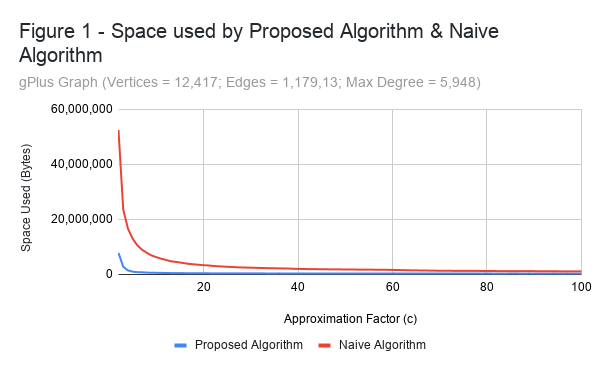
\includegraphics[scale=1]{img/Figure1.png}
	\end{tabular}\end{center}	
  \end{block}
  \end{column}
  \begin{column}{0.422\linewidth}
  \begin{block}{\Large 4. Further Aims}
  \begin{itemize}
  \item Perform tests on different size graphs for the same approximation factor.
  \item Perform tests on different density graphs for the same approximation factor.
  \item Implement the proposed algorithm for \textit{Insertion-Deletion Streams}.
  \item Investigate an application of these algorithms.
  \end{itemize}
	\begin{center}\begin{tabular}{c}
	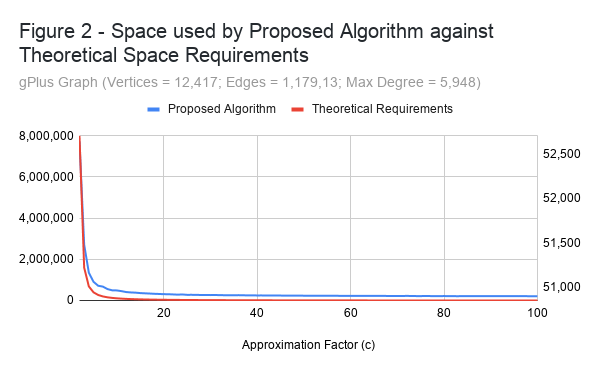
\includegraphics[scale=1]{img/Figure2.png}
	\end{tabular}\end{center}
  \end{block}
  \end{column}
\end{columns}

\vfill

\end{frame}

% -----------------------------------------------------------------------------

\end{document}



